
%|  Name  | TODO | ONGOING | DONE |
%|--------|------|---------|------|
%| Dana   | x    |         |      |
%| Gerd   |      |         | x    |
%| Glenn  |      |         |   x  |
%| Jordan | x    |         |      |
%| Luke   | x    |         |      |
%| Matt   |      |         |  x   |
%| Neil   | x    |         |      |
%| Scot   |     |         |   x   |

%\todo[inline]{Owner: Gerd -- Priority: High -- Effort: M -- Completion: 100\%}

Throughout this tour, we describe the different user-controllable caching and buffering facilities. Figure~\ref{fig:cache-buf} shows an overview of these facilities.

\begin{figure}[bh]
\centering
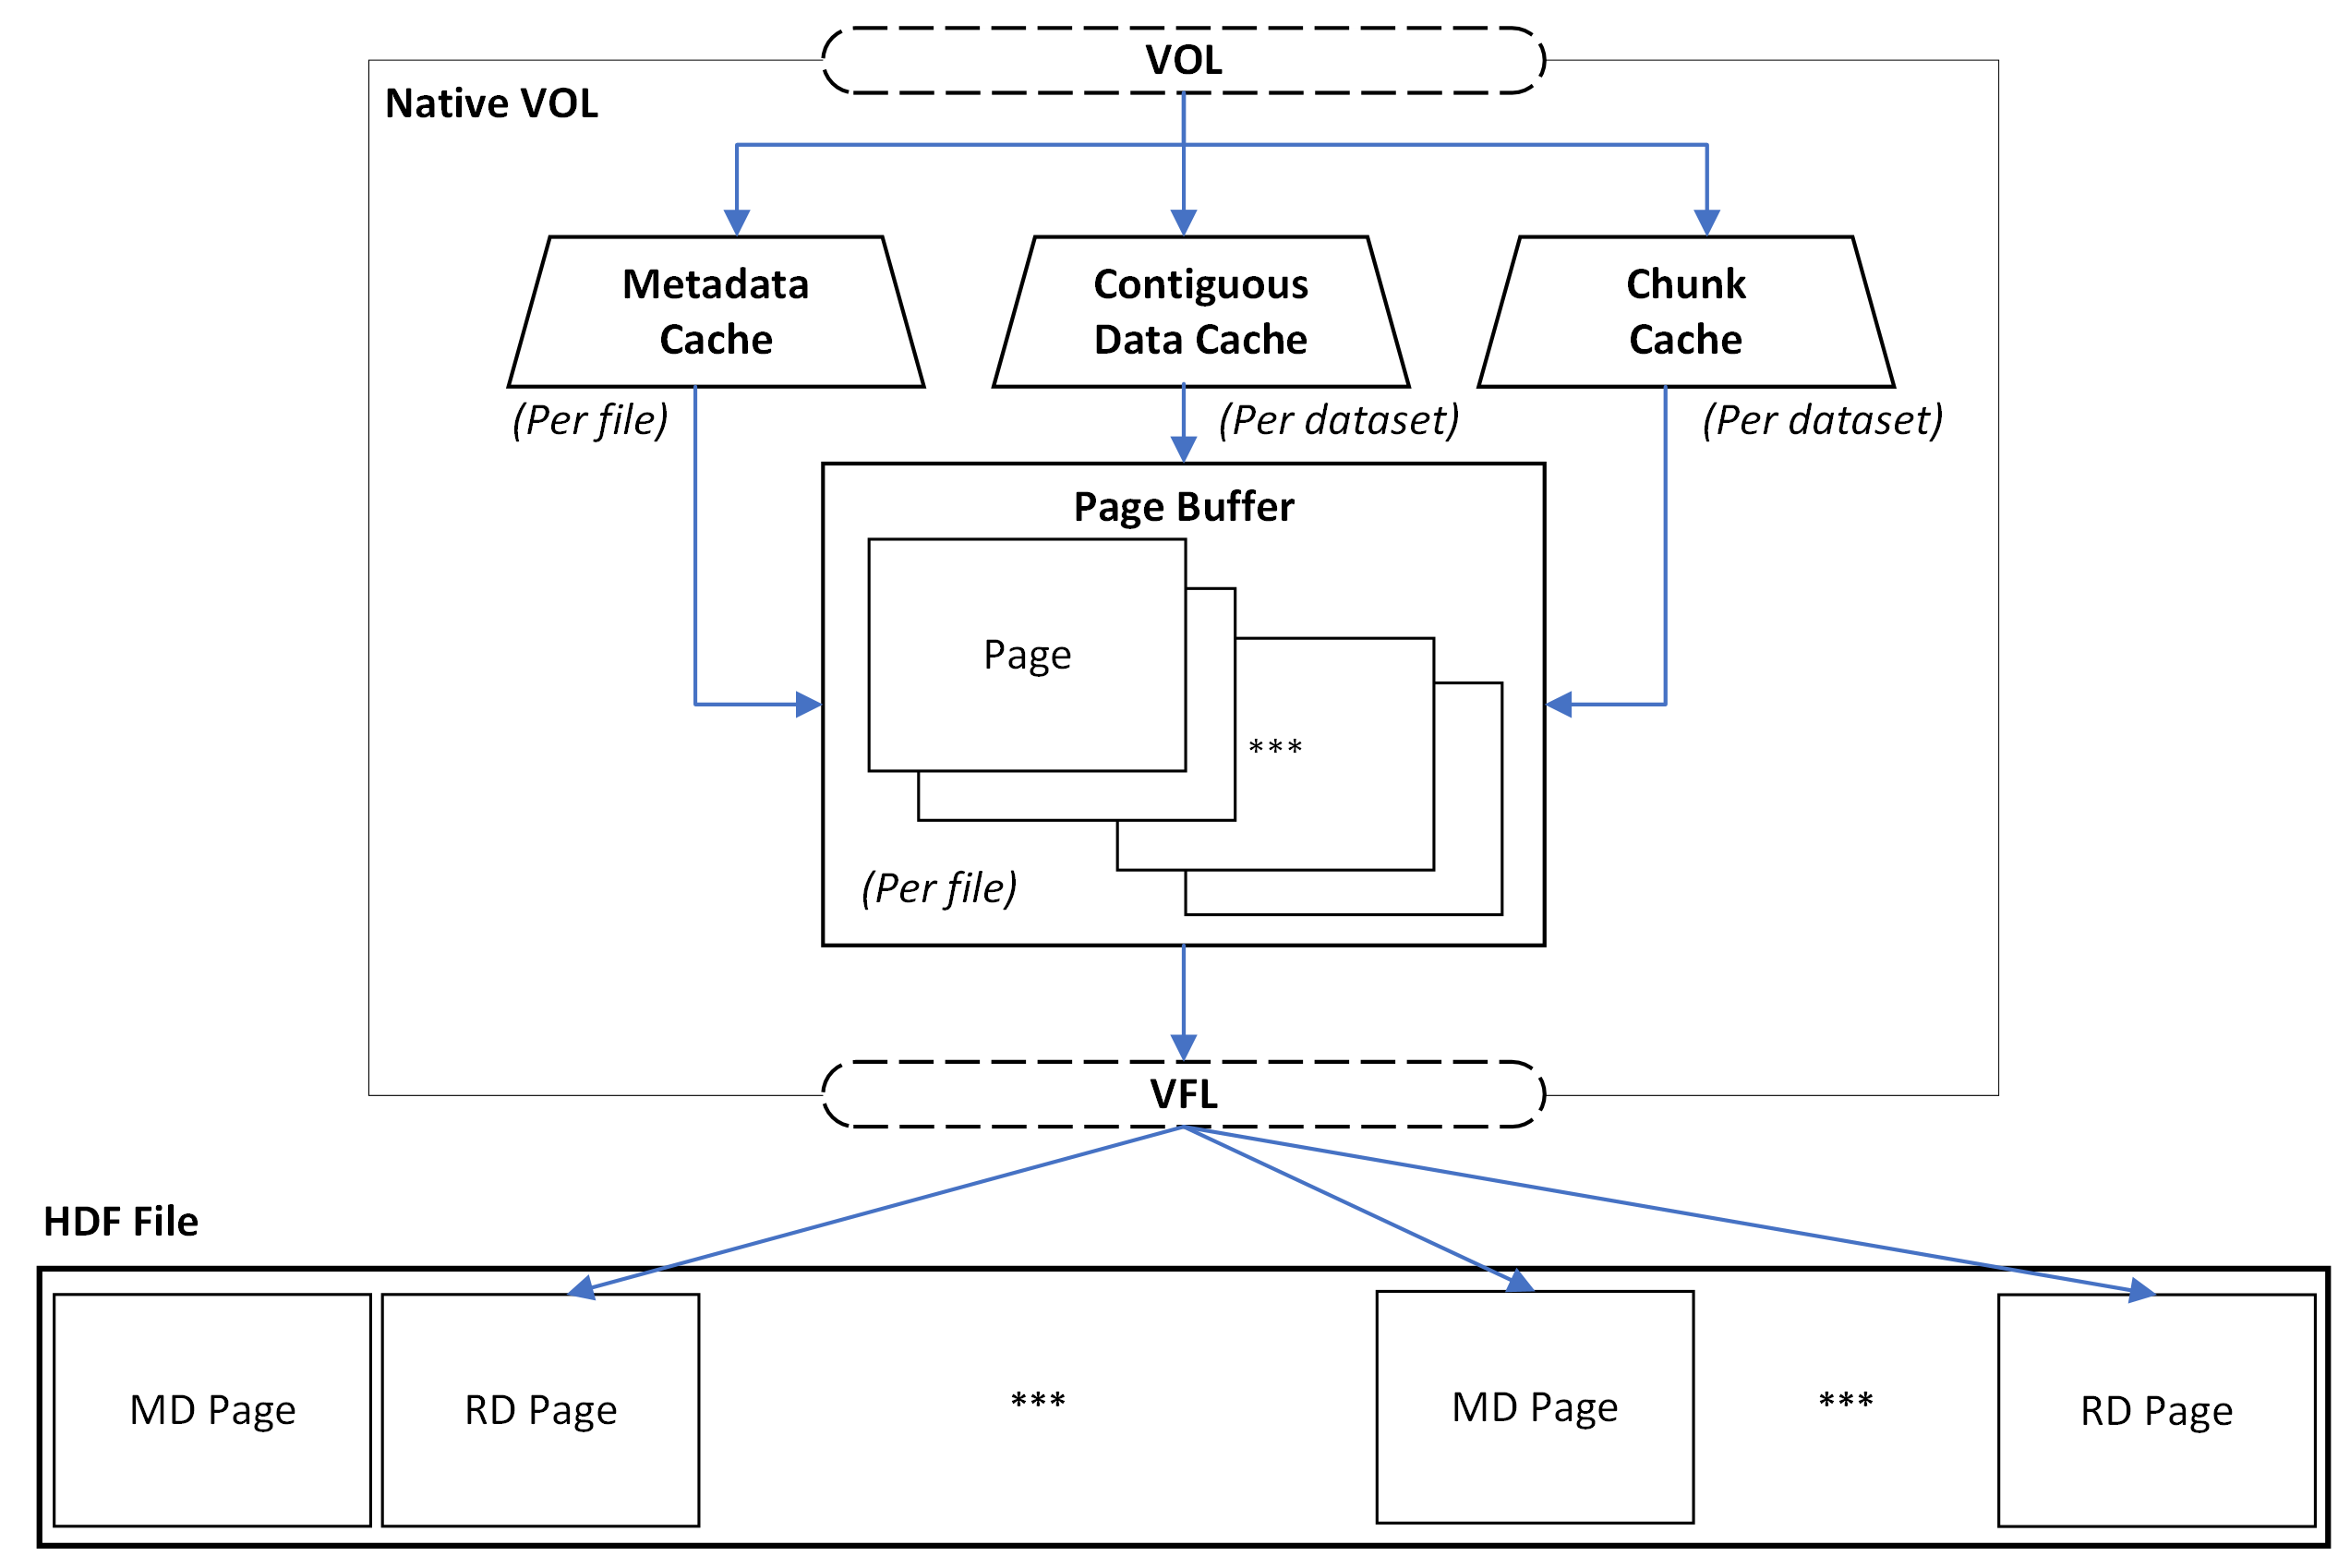
\includegraphics[width=\textwidth]{images/Caches to caches.png}
\caption{Native VOL caching and buffering.}
\label{fig:cache-buf}
\end{figure}

There are four architectural elements in the native VOL that implement caching or buffering functionality.

\begin{itemize}
    \item \textbf{Metadata cache:} We have encountered the metadata cache in Sections~\ref{sec:tour2} and~\ref{sec:tour3}.
    \item \textbf{Contiguous data cache:}  Frequently accessed contiguous dataset regions can be held in memory to minimize small I/O for datasets with contiguous storage layouts.
    \item \textbf{Chunk cache:} Frequently accessed chunks can be held in memory to minimize chunk I/O for datasets with chunked storage layouts.
    \item \textbf{Page buffer:} Since HDF5 library version 1.10.0, file space can be managed and I/O operations performed in fixed-size pages. This so-called `paged aggregation' or `paged allocation' scheme is most effective when combined with a page buffer.
\end{itemize}

The cache vs. buffer terminology in the native VOL is a little murky. The term `cache' is usually applied to a data structure that, in its implementation, uses several slots to which specific entries are assigned and which is controlled by a hash function that might have a degree of associativity. Typically, there is also an entry eviction or prefetch policy defined. The metadata and chunk caches are caches in that sense. The contiguous data cache (or sieve buffer), not so much. The native VOL caches and the page buffer gather internal usage statistics, which can be used to assess their effectiveness for particular applications.

During this tour, we take a \textit{qualitative} look at several examples where we will see the different facilities in action. This is, however, not the place to quantify the actual performance impact. This is highly problem size and access pattern-dependent, and the significant influence of the operating system's memory page cache cannot be overestimated.

\subsection{``Raw" Data (RD) and Metadata (MD)}

We already encountered the metadata cache in tours~\ref{sec:tour2} and~\ref{sec:tour3}. Before looking at a specific example, let's remind ourselves what, in this context, we mean by metadata versus raw data.

\begin{center}
\begin{tabular}{ | m{20em} | m{20em} | }
  \hline
  \textbf{Metadata} & \textbf{Raw Data} \\ \hline
  \begin{itemize}
      \item Entries enumerated in \texttt{H5AC\_type\_t}
      \item File pages filled with metadata
  \end{itemize}
  &
  \begin{itemize}
  \item Contiguous regions of datasets
  \item Dataset chunks
  \item File pages filled with raw data
  \end{itemize} \\ 
  \hline
\end{tabular}
\end{center}

\texttt{H5AC\_type\_t} is defined in \texttt{H5ACprivate.h}, and, with a few exceptions, contains many of the metadata items found in the HDF5 file format specification~\cite{ffmt} such as file superblock, symbol table nodes, local heaps, object headers, B-tree nodes, etc. If a paged allocation is used and a page buffer is present (see section~\ref{sub-sec:page-buf}), file space is managed in fixed-size pages containing either metadata or raw data. The page buffer is a memory region set aside to store a list of frequently accessed file pages.

\subsection{The mighty metadata cache (MDC)}

To simulate the impact of an improperly configured (or altogether absent) MDC, we perform a set of metadata-intensive operations and arbitrarily ``throttle" the MDC via \texttt{H5Pset\_mdc\_config()} as shown in listing~\ref{lst:no-mdc}. The code creates and then deletes 50,000 subgroups in separate loops and then creates another 25,000 subgroups. Most of the metadata will be local heaps and symbol tables from all these groups. Running the code with the \texttt{throttle} argument curtails the metadata cache size to 1KiB. With the throttled configuration, the code runs more than five times slower than the default configuration. Reviewing the Callgrind profile, this increase is almost proportional to the increase in \texttt{H5C\_\_flush\_single\_entry()} calls from \texttt{H5C\_\_make\_space\_in\_cache()} (429,136 to 1,873,837 with \texttt{throttle}).

\begin{listing}
\centering
\caption{Tiny MDC.}
\label{lst:no-mdc}
\begin{minted}[linenos]{C}
#include "common.h"
void set_mdc_config(H5AC_cache_config_t *config)
{
    config->version                = H5AC__CURR_CACHE_CONFIG_VERSION;
    config->rpt_fcn_enabled        = 0;
    config->open_trace_file        = 0;
    config->close_trace_file       = 0;
    config->evictions_enabled      = 1;
    config->dirty_bytes_threshold  = 1024;
    config->max_size               = 1024;
    config->min_size               = 1024;
    config->set_initial_size       = 0;
    config->epoch_length           = 50000;
    config->incr_mode              = H5C_incr__off;
}
int main(int argc, char** argv) {
    H5AC_cache_config_t mdc_config;
    hid_t fapl = H5Pcreate(H5P_FILE_ACCESS);
    if (argc > 1 && strcmp(argv[1], "throttle") == 0) {
        set_mdc_config(&mdc_config);
        H5Pset_mdc_config(fapl, &mdc_config);
    }
    hid_t file=H5Fcreate("group.1.h5",H5F_ACC_TRUNC,H5P_DEFAULT,fapl);
    hid_t group1 = H5Gcreate(file, "group1", H5P_DEFAULTx3);
    char data[16] = "subgroup XXXXX";
    for (size_t i = 0; i < 50000; ++i) {
        snprintf(data + 8, 6, "%05zu", i);
        H5Gclose(H5Gcreate(group1, data, H5P_DEFAULTx3));}
    for (size_t i = 0; i < 50000; i += 2) {
        snprintf(data + 8, 6, "%05zu", i);
        H5Gunlink(group1, data);}
    H5Gclose(group1);
    hid_t group2 = H5Gcreate(file, "group2", H5P_DEFAULTx3);
    for (size_t i = 0; i < 25000; ++i) {
        snprintf(data + 8, 6, "%05zu", i);
        H5Gclose(H5Gcreate(group2, data, H5P_DEFAULTx3));}
    H5Gclose(group2);
    H5Fclose(file);
    return 0;
}
\end{minted}
\end{listing}


\subsection{Caching ``raw" data}

\subsubsection{Contiguous data cache (a.k.a. data sieve buffer)}

Data sieving~\cite{thakur1999} is a common technique to make a few large, contiguous requests to the file system, even if the user’s request consists of several small, non-contiguous accesses, e.g., point or hyperslab selections. The native VOL uses this technique for datasets with contiguous layouts. The definition of the so-called `raw data contiguous data cache' can be found in \texttt{H5Dpkg.h} and is repeated in listing~\ref{lst:rdcdc}. \texttt{sieve\_loc} is the offset of the sieve in the HDF5 file, \texttt{sieve\_size} is the used size of the total \texttt{sieve\_buf\_size}, and \texttt{sieve\_dirty} tracks the sieve buffer's modification status. The sieve buffer size can be controlled at the file level(!) via \texttt{H5Pset\_sieve\_buf\_size()}.

\begin{listing}
\centering
\caption{Raw data contiguous data cache (\texttt{rdcdc}!).}
\label{lst:rdcdc}
\begin{minted}[linenos]{C}
typedef struct H5D_rdcdc_t {
    unsigned char *sieve_buf;
    haddr_t        sieve_loc;
    size_t         sieve_size;
    size_t         sieve_buf_size;
    bool           sieve_dirty;
} H5D_rdcdc_t;
\end{minted}
\end{listing}

\subsubsection{Chunk cache}

The chunk cache is defined as struct \texttt{H5D\_rdcc\_t} in \texttt{H5Dpkg.h}, and the definition is too long to be reproduced here. Like most caches, it has a set of slots for cache entries, an auxiliary doubly-linked list to implement an eviction strategy based on LRU or similar, and performance counters for statistics.

To see the chunk cache in action and the side effects of an undersized chunk cache, we have created the example in listing~\ref{lst:no-ccache}. In this example, we update single elements on different chunks, forcing chunk cache evictions if the chunk cache cannot hold all chunks. The dataset has 1,048,576 32-bit integer elements allocated across four chunks. The default chunk cache size is 1MiB, which can hold a single chunk. In every loop iteration, we update an element on a different chunk, evicting the current chunk. Passing the \texttt{cache-all} argument to the program increases the chunk cache to 4MiB, which can hold all four chunks in the chunk cache without evictions. The Callgrind profiles' main difference is 100 calls to \texttt{H5D\_\_chunk\_cache\_prune()} with the default (undersized) chunk cache, which we expected. Because of the OS's page cache, the actual performance difference is negligible for the small chunk sizes in this example. However, this would not be true for larger datasets, chunks, other access patterns, and system loads.

\begin{listing}
\centering
\caption{Undersized chunk cache.}
\label{lst:no-ccache}
\begin{minted}[linenos]{C}
#include "common.h"
int main(int argc, char** argv)
{
    hid_t file = H5Fcreate("data.5.h5", H5F_ACC_TRUNC, H5P_DEFAULTx2);
    hid_t fspace = H5Screate_simple(1, (hsize_t[]){_1MIB}, NULL);
    hid_t dcpl = H5Pcreate(H5P_DATASET_CREATE);
    H5Pset_chunk(dcpl, 1, (hsize_t[]){_256KIB});
    hid_t dapl = H5Pcreate(H5P_DATASET_ACCESS);
    if (argc > 1 && strcmp(argv[1], "cache-all") == 0)
        H5Pset_chunk_cache(dapl, H5D_CHUNK_CACHE_NSLOTS_DEFAULT, _4MIB,
            H5D_CHUNK_CACHE_W0_DEFAULT);
    hid_t dset = H5Dcreate(file, "data", H5T_NATIVE_INT, fspace,
        H5P_DEFAULT, dcpl, dapl);
    hid_t mspace = H5Screate_simple(1, (hsize_t[]){1}, NULL);
    H5Sselect_elements(mspace, H5S_SELECT_SET, 1, (hsize_t[]){0});
    
    for (int i = 0; i < 100; ++i)
    {
        H5Sselect_elements(fspace, H5S_SELECT_SET, 1,
            (hsize_t[]){(i%4)*_256KIB+i});
        H5Dwrite(dset, H5T_NATIVE_INT, mspace, fspace, H5P_DEFAULT, &i);
    }
    H5Sclose(mspace);
    H5Pclose(dapl);     
    H5Pclose(dcpl);  
    H5Dclose(dset);
    H5Sclose(fspace);
    H5Fclose(file);
    return 0;
}
\end{minted}
\end{listing}

\subsection{Page buffering}\label{sub-sec:page-buf}

In HDF5 library release 1.10.0, a new file space management strategy, \textit{paged aggregation}, that aggregates small metadata and raw data allocations into constant-sized, well-aligned pages was introduced~\cite{rfc20120523}. Paged aggregation combined with \textit{page buffering}~\cite{rfc20150709} allows more efficient I/O accesses.

To see the paged aggregation/page buffering combination in action, we have modified listing~\ref{lst:no-ccache} and updated the file creation and access property lists to arrive at listing~\ref{lst:pages}. We have updated the behavior of the \texttt{cache-all} argument to bump the page buffer size from 1MiB to 8MiB. The latter can accommodate all file pages. Again, looking at the differences in the Callgrind profiles, the differences are clear to see. A good measure of the effectiveness of paged aggregation and page buffering is to look at the number of \texttt{H5PB[read,write]()} and \texttt{pwrite()} calls.

\texttt{H5PBwrite()} writes data into the page buffer. If the page exists in the cache, update it; otherwise, read it from the disk, update it, and insert it into the cache.

\texttt{H5PBread()} reads in the data from the page containing it if it exists in the page buffer; otherwise, it reads the page through the VFD.

The number of \texttt{pwrite()} calls indicates the I/O traffic the OS sees from the application.

\begin{listing}
\centering
\caption{Paged allocation and page buffering.}
\label{lst:pages}
\begin{minted}[linenos]{C}
#include "common.h"
int main(int argc, char** argv)
{
    hid_t fcpl = H5Pcreate(H5P_FILE_CREATE);
    H5Pset_file_space_strategy(fcpl, H5F_FSPACE_STRATEGY_PAGE, 1, _4KIB);
    H5Pset_file_space_page_size(fcpl, _4KIB);
    hid_t fapl = H5Pcreate(H5P_FILE_ACCESS);
    if (argc > 1 && strcmp(argv[1], "cache-all") == 0)
        H5Pset_page_buffer_size(fapl, _8MIB, 0, 0);
    else
        H5Pset_page_buffer_size(fapl, _1MIB, 0, 0);

    hid_t file = H5Fcreate("data.6.h5", H5F_ACC_TRUNC, fcpl, fapl);
    hid_t fspace = H5Screate_simple(1, (hsize_t[]){_1MIB}, NULL);
    hid_t dcpl = H5Pcreate(H5P_DATASET_CREATE);
    H5Pset_chunk(dcpl, 1, (hsize_t[]){_256KIB});
    hid_t dapl = H5Pcreate(H5P_DATASET_ACCESS);
    if (argc > 1 && strcmp(argv[1], "cache-all") == 0)
        H5Pset_chunk_cache(dapl, H5D_CHUNK_CACHE_NSLOTS_DEFAULT, _4MIB,
            H5D_CHUNK_CACHE_W0_DEFAULT);

    hid_t dset = H5Dcreate(file, "data", H5T_NATIVE_INT, fspace,
        H5P_DEFAULT, dcpl, dapl);
    hid_t mspace = H5Screate_simple(1, (hsize_t[]){1}, NULL);
    H5Sselect_elements(mspace, H5S_SELECT_SET, 1, (hsize_t[]){0});
    
    for (int i = 0; i < 100; ++i)
    {
        H5Sselect_elements(fspace, H5S_SELECT_SET, 1,
            (hsize_t[]){(i%4)*_256KIB+i});
        H5Dwrite(dset, H5T_NATIVE_INT, mspace, fspace, H5P_DEFAULT, &i);
    }
    H5Sclose(mspace);
    H5Pclose(dapl);     
    H5Pclose(dcpl);  
    H5Dclose(dset);
    H5Sclose(fspace);
    H5Fclose(file);
    return 0;
}
\end{minted}
\end{listing}

The call counts without and with the \texttt{cache-all} argument are shown in parentheses.
\begin{itemize}
    \item \texttt{H5PBwrite()} (114 / 18)
    \item \texttt{H5PBread()} (96 / 0)
    \item \texttt{pwrite()} (102 / 6)
\end{itemize}

The drop in call counts is significant. Again, depending on the problem size, the effectiveness of the OS page cache will intervene, and the actual performance difference between the two scenarios may not be near what the counts suggest.

\subsection{Summary}

During this tour, we looked at four user-controllable caching and buffering facilities for metadata and raw data in the native VOL. They are effective on paper, and the default configurations might often be sufficient. Ideally, these features would be adaptive and self-tuning since their inclusion in any code base is fraught with portability and maintenance issues. Finally, three of the four facilities also capture statistics that can be used to assess their effectiveness in real-life scenarios.